\documentclass[]{book}
\usepackage{lmodern}
\usepackage{amssymb,amsmath}
\usepackage{ifxetex,ifluatex}
\usepackage{fixltx2e} % provides \textsubscript
\ifnum 0\ifxetex 1\fi\ifluatex 1\fi=0 % if pdftex
  \usepackage[T1]{fontenc}
  \usepackage[utf8]{inputenc}
\else % if luatex or xelatex
  \ifxetex
    \usepackage{mathspec}
  \else
    \usepackage{fontspec}
  \fi
  \defaultfontfeatures{Ligatures=TeX,Scale=MatchLowercase}
\fi
% use upquote if available, for straight quotes in verbatim environments
\IfFileExists{upquote.sty}{\usepackage{upquote}}{}
% use microtype if available
\IfFileExists{microtype.sty}{%
\usepackage{microtype}
\UseMicrotypeSet[protrusion]{basicmath} % disable protrusion for tt fonts
}{}
\usepackage{hyperref}
\hypersetup{unicode=true,
            pdftitle={The Surgical Informatics Cookbook},
            pdfauthor={Surgical Informatics, University of Edinburgh},
            pdfborder={0 0 0},
            breaklinks=true}
\urlstyle{same}  % don't use monospace font for urls
\usepackage{natbib}
\bibliographystyle{apalike}
\usepackage{color}
\usepackage{fancyvrb}
\newcommand{\VerbBar}{|}
\newcommand{\VERB}{\Verb[commandchars=\\\{\}]}
\DefineVerbatimEnvironment{Highlighting}{Verbatim}{commandchars=\\\{\}}
% Add ',fontsize=\small' for more characters per line
\usepackage{framed}
\definecolor{shadecolor}{RGB}{248,248,248}
\newenvironment{Shaded}{\begin{snugshade}}{\end{snugshade}}
\newcommand{\AlertTok}[1]{\textcolor[rgb]{0.94,0.16,0.16}{#1}}
\newcommand{\AnnotationTok}[1]{\textcolor[rgb]{0.56,0.35,0.01}{\textbf{\textit{#1}}}}
\newcommand{\AttributeTok}[1]{\textcolor[rgb]{0.77,0.63,0.00}{#1}}
\newcommand{\BaseNTok}[1]{\textcolor[rgb]{0.00,0.00,0.81}{#1}}
\newcommand{\BuiltInTok}[1]{#1}
\newcommand{\CharTok}[1]{\textcolor[rgb]{0.31,0.60,0.02}{#1}}
\newcommand{\CommentTok}[1]{\textcolor[rgb]{0.56,0.35,0.01}{\textit{#1}}}
\newcommand{\CommentVarTok}[1]{\textcolor[rgb]{0.56,0.35,0.01}{\textbf{\textit{#1}}}}
\newcommand{\ConstantTok}[1]{\textcolor[rgb]{0.00,0.00,0.00}{#1}}
\newcommand{\ControlFlowTok}[1]{\textcolor[rgb]{0.13,0.29,0.53}{\textbf{#1}}}
\newcommand{\DataTypeTok}[1]{\textcolor[rgb]{0.13,0.29,0.53}{#1}}
\newcommand{\DecValTok}[1]{\textcolor[rgb]{0.00,0.00,0.81}{#1}}
\newcommand{\DocumentationTok}[1]{\textcolor[rgb]{0.56,0.35,0.01}{\textbf{\textit{#1}}}}
\newcommand{\ErrorTok}[1]{\textcolor[rgb]{0.64,0.00,0.00}{\textbf{#1}}}
\newcommand{\ExtensionTok}[1]{#1}
\newcommand{\FloatTok}[1]{\textcolor[rgb]{0.00,0.00,0.81}{#1}}
\newcommand{\FunctionTok}[1]{\textcolor[rgb]{0.00,0.00,0.00}{#1}}
\newcommand{\ImportTok}[1]{#1}
\newcommand{\InformationTok}[1]{\textcolor[rgb]{0.56,0.35,0.01}{\textbf{\textit{#1}}}}
\newcommand{\KeywordTok}[1]{\textcolor[rgb]{0.13,0.29,0.53}{\textbf{#1}}}
\newcommand{\NormalTok}[1]{#1}
\newcommand{\OperatorTok}[1]{\textcolor[rgb]{0.81,0.36,0.00}{\textbf{#1}}}
\newcommand{\OtherTok}[1]{\textcolor[rgb]{0.56,0.35,0.01}{#1}}
\newcommand{\PreprocessorTok}[1]{\textcolor[rgb]{0.56,0.35,0.01}{\textit{#1}}}
\newcommand{\RegionMarkerTok}[1]{#1}
\newcommand{\SpecialCharTok}[1]{\textcolor[rgb]{0.00,0.00,0.00}{#1}}
\newcommand{\SpecialStringTok}[1]{\textcolor[rgb]{0.31,0.60,0.02}{#1}}
\newcommand{\StringTok}[1]{\textcolor[rgb]{0.31,0.60,0.02}{#1}}
\newcommand{\VariableTok}[1]{\textcolor[rgb]{0.00,0.00,0.00}{#1}}
\newcommand{\VerbatimStringTok}[1]{\textcolor[rgb]{0.31,0.60,0.02}{#1}}
\newcommand{\WarningTok}[1]{\textcolor[rgb]{0.56,0.35,0.01}{\textbf{\textit{#1}}}}
\usepackage{longtable,booktabs}
\usepackage{graphicx,grffile}
\makeatletter
\def\maxwidth{\ifdim\Gin@nat@width>\linewidth\linewidth\else\Gin@nat@width\fi}
\def\maxheight{\ifdim\Gin@nat@height>\textheight\textheight\else\Gin@nat@height\fi}
\makeatother
% Scale images if necessary, so that they will not overflow the page
% margins by default, and it is still possible to overwrite the defaults
% using explicit options in \includegraphics[width, height, ...]{}
\setkeys{Gin}{width=\maxwidth,height=\maxheight,keepaspectratio}
\IfFileExists{parskip.sty}{%
\usepackage{parskip}
}{% else
\setlength{\parindent}{0pt}
\setlength{\parskip}{6pt plus 2pt minus 1pt}
}
\setlength{\emergencystretch}{3em}  % prevent overfull lines
\providecommand{\tightlist}{%
  \setlength{\itemsep}{0pt}\setlength{\parskip}{0pt}}
\setcounter{secnumdepth}{5}
% Redefines (sub)paragraphs to behave more like sections
\ifx\paragraph\undefined\else
\let\oldparagraph\paragraph
\renewcommand{\paragraph}[1]{\oldparagraph{#1}\mbox{}}
\fi
\ifx\subparagraph\undefined\else
\let\oldsubparagraph\subparagraph
\renewcommand{\subparagraph}[1]{\oldsubparagraph{#1}\mbox{}}
\fi

%%% Use protect on footnotes to avoid problems with footnotes in titles
\let\rmarkdownfootnote\footnote%
\def\footnote{\protect\rmarkdownfootnote}

%%% Change title format to be more compact
\usepackage{titling}

% Create subtitle command for use in maketitle
\providecommand{\subtitle}[1]{
  \posttitle{
    \begin{center}\large#1\end{center}
    }
}

\setlength{\droptitle}{-2em}

  \title{The Surgical Informatics Cookbook}
    \pretitle{\vspace{\droptitle}\centering\huge}
  \posttitle{\par}
    \author{Surgical Informatics, University of Edinburgh}
    \preauthor{\centering\large\emph}
  \postauthor{\par}
      \predate{\centering\large\emph}
  \postdate{\par}
    \date{2019-10-01}

\usepackage{booktabs}

\begin{document}
\maketitle

{
\setcounter{tocdepth}{1}
\tableofcontents
}
\hypertarget{intro}{%
\chapter{Introduction}\label{intro}}

\hypertarget{how-to-contribute}{%
\section{How to contribute}\label{how-to-contribute}}

(Steps 1. to 5. only need to be done once - to set-up.)

\begin{enumerate}
\def\labelenumi{\arabic{enumi}.}
\item
  Connect your RStudio and GitHub using these instructions, only up to ``Create new project'' is necessary here (the repository/project already exists):
  \url{https://www.datasurg.net/2015/07/13/rstudio-and-github/}
\item
  Get your GitHub account added to the surgicalinformatics organisation on GitHub (ask Riinu/Ewen):
  \url{https://github.com/SurgicalInformatics}
\item
  Open the terminal on argonaut, go to your home folder (just \texttt{cd} will default to taking you home). If the prompt says \texttt{username@argonaut:\textasciitilde{}\$} that means you're home - \texttt{\textasciitilde{}} means user's home.
\item
  In the terminal, do \texttt{git\ clone\ git@github.com:SurgicalInformatics/cookbook.git}.
\item
  Look at the Files tab - a new folder called \texttt{cookbook} should have appeared at the bottom. Click on it and open the cookbook.Rproj file.
\item
  Add your thing by editing the appropriate .Rmd file - there's one for each chapter. Use the Build tab to Build your changes into a book.
\item
  If anyone has pushed since you cloned/last pulled (hopefully they've not been working on the exact same chapter): click on More - Clean All. Then Pull from the Git tab. This only cleans the output files - html and PDF, it will not touch the changes you've made in the .Rmd file.
\item
  Then Build Book again - this will include the new changes you pulled as well as your changes.
\item
  Git tab - commit everything, Push quickly before anyone else does or you'll have to go back to step 7. You can check for new pushed commits here: \url{https://github.com/SurgicalInformatics/cookbook/commits/master} Alternatively there's no harm in clicking the Pull button again - it should then say ``Already up-to-date''.
\end{enumerate}

\begin{quote}
Pro tip: instead of clicking on every single file in the Git tab, go to the terminal, \texttt{cd\ cookbook} to go to the project folder if still home, and do \texttt{git\ add\ -A} which is the same thing. Still need to Commit though!
\end{quote}

\textbf{10. Have fun!}

\hypertarget{rules-of-posting}{%
\section{Rules of posting}\label{rules-of-posting}}

Rules of how to post here.

\hypertarget{indexing}{%
\section{Indexing}\label{indexing}}

\hypertarget{index}{%
\subsection{Index}\label{index}}

Bold index headings:\\
\texttt{\textbackslash{}index\{linear\ regression@\textbackslash{}textbf\{linear\ regression\}\}} (ticks in .Rmd file are excluded when actually using)

Sub-entries of bold headings:\\
\texttt{\textbackslash{}index\{linear\ regression@\textbackslash{}textbf\{linear\ regression\}!diagnostics\}}

Stand-alone entries:\\
\texttt{\textbackslash{}index\{linear\ regression\}}

\hypertarget{chapter-and-section-references}{%
\subsection{Chapter and section references}\label{chapter-and-section-references}}

You can label chapter and section titles using \texttt{\{\#label\}} after them, e.g., we can reference Chapter \texttt{\textbackslash{}@ref(intro)} (ticks in .Rmd are excluded when actually using). If you do not manually label them, there will be automatic labels anyway, e.g., Chapter \texttt{\textbackslash{}@ref(methods)}.

\hypertarget{figure-and-table-references}{%
\subsection{Figure and table references}\label{figure-and-table-references}}

Figures and tables with captions will be placed in \texttt{figure} and \texttt{table} environments, respectively.

\begin{Shaded}
\begin{Highlighting}[]
\KeywordTok{par}\NormalTok{(}\DataTypeTok{mar =} \KeywordTok{c}\NormalTok{(}\DecValTok{4}\NormalTok{, }\DecValTok{4}\NormalTok{, }\FloatTok{.1}\NormalTok{, }\FloatTok{.1}\NormalTok{))}
\KeywordTok{plot}\NormalTok{(pressure, }\DataTypeTok{type =} \StringTok{'b'}\NormalTok{, }\DataTypeTok{pch =} \DecValTok{19}\NormalTok{)}
\end{Highlighting}
\end{Shaded}

\begin{figure}

{\centering 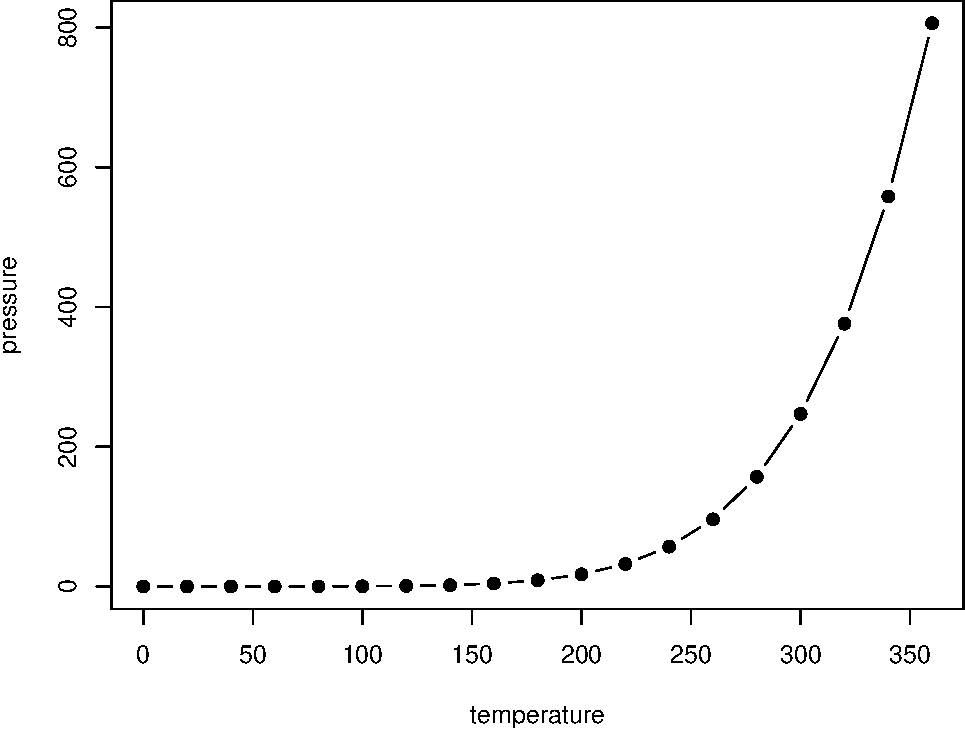
\includegraphics[width=0.8\linewidth]{cookbook_files/figure-latex/nice-fig-1} 

}

\caption{Here is a nice figure!}\label{fig:nice-fig}
\end{figure}

Reference a figure by its code chunk label with the \texttt{fig:} prefix, e.g., see Figure \texttt{\textbackslash{}@ref(fig:nice-fig)}. Similarly, you can reference tables generated from \texttt{knitr::kable()}, e.g., see Table \texttt{\textbackslash{}@ref(tab:nice-tab)}.

\begin{Shaded}
\begin{Highlighting}[]
\NormalTok{knitr}\OperatorTok{::}\KeywordTok{kable}\NormalTok{(}
  \KeywordTok{head}\NormalTok{(iris, }\DecValTok{20}\NormalTok{), }\DataTypeTok{caption =} \StringTok{'Here is a nice table!'}\NormalTok{,}
  \DataTypeTok{booktabs =} \OtherTok{TRUE}
\NormalTok{)}
\end{Highlighting}
\end{Shaded}

\begin{table}

\caption{\label{tab:nice-tab}Here is a nice table!}
\centering
\begin{tabular}[t]{rrrrl}
\toprule
Sepal.Length & Sepal.Width & Petal.Length & Petal.Width & Species\\
\midrule
5.1 & 3.5 & 1.4 & 0.2 & setosa\\
4.9 & 3.0 & 1.4 & 0.2 & setosa\\
4.7 & 3.2 & 1.3 & 0.2 & setosa\\
4.6 & 3.1 & 1.5 & 0.2 & setosa\\
5.0 & 3.6 & 1.4 & 0.2 & setosa\\
\addlinespace
5.4 & 3.9 & 1.7 & 0.4 & setosa\\
4.6 & 3.4 & 1.4 & 0.3 & setosa\\
5.0 & 3.4 & 1.5 & 0.2 & setosa\\
4.4 & 2.9 & 1.4 & 0.2 & setosa\\
4.9 & 3.1 & 1.5 & 0.1 & setosa\\
\addlinespace
5.4 & 3.7 & 1.5 & 0.2 & setosa\\
4.8 & 3.4 & 1.6 & 0.2 & setosa\\
4.8 & 3.0 & 1.4 & 0.1 & setosa\\
4.3 & 3.0 & 1.1 & 0.1 & setosa\\
5.8 & 4.0 & 1.2 & 0.2 & setosa\\
\addlinespace
5.7 & 4.4 & 1.5 & 0.4 & setosa\\
5.4 & 3.9 & 1.3 & 0.4 & setosa\\
5.1 & 3.5 & 1.4 & 0.3 & setosa\\
5.7 & 3.8 & 1.7 & 0.3 & setosa\\
5.1 & 3.8 & 1.5 & 0.3 & setosa\\
\bottomrule
\end{tabular}
\end{table}

\hypertarget{citations}{%
\subsection{Citations}\label{citations}}

You can write citations, too. For example, we are using the \textbf{bookdown} package \citep{R-bookdown} in this sample book, which was built on top of R Markdown and \textbf{knitr} \citep{xie2015}.

\hypertarget{snippets}{%
\chapter{Snippets}\label{snippets}}

Random useful snippets that do not fit anywhere else.

\hypertarget{working-with-chis}{%
\section{Working with CHIs}\label{working-with-chis}}

Here are 4 functions for CHIs that could even be put in a small package.
The Community Health Index (CHI) is a population register, which is used in Scotland for health care purposes.
The CHI number uniquely identifies a person on the index.

\hypertarget{chi_dob---extract-date-of-birth-from-chi}{%
\subsection{\texorpdfstring{\texttt{chi\_dob()} - Extract date of birth from CHI}{chi\_dob() - Extract date of birth from CHI}}\label{chi_dob---extract-date-of-birth-from-chi}}

Note \texttt{cutoff\_2000}.
As CHI has only a two digit year, need to decide whether year is 1900s or 2000s.
I don't think there is a formal way of determining this.

\begin{Shaded}
\begin{Highlighting}[]
\KeywordTok{library}\NormalTok{(dplyr)}
\NormalTok{chi =}\StringTok{ }\KeywordTok{c}\NormalTok{(}\StringTok{"1009701234"}\NormalTok{, }\StringTok{"1811431232"}\NormalTok{, }\StringTok{"1304496368"}\NormalTok{)}
\CommentTok{# These CHIs are not real. }
\CommentTok{# The first is invalid, two and three are valid. }

\CommentTok{# Cut-off any thing before that number is considered 2000s}
\CommentTok{# i.e. at cutoff_2000 = 20, "18" is considered 2018, rather than 1918. }
\NormalTok{chi_dob =}\StringTok{ }\ControlFlowTok{function}\NormalTok{(.data, }\DataTypeTok{cutoff_2000 =} \DecValTok{20}\NormalTok{)\{}
\NormalTok{  .data }\OperatorTok\StringTok{ }
\StringTok{    }\NormalTok{stringr}\OperatorTok{::}\KeywordTok{str_extract}\NormalTok{(}\StringTok{".\{6\}"}\NormalTok{) }\OperatorTok\StringTok{ }
\StringTok{    }\NormalTok{lubridate}\OperatorTok{::}\KeywordTok{parse_date_time2}\NormalTok{(}\StringTok{"dmy"}\NormalTok{, }\DataTypeTok{cutoff_2000 =}\NormalTok{ cutoff_}\DecValTok{2000}\NormalTok{) }\OperatorTok\StringTok{ }
\StringTok{    }\NormalTok{lubridate}\OperatorTok{::}\KeywordTok{as_date}\NormalTok{() }\CommentTok{# Make Date object, rather than POSIXct}
\NormalTok{\}}

\KeywordTok{chi_dob}\NormalTok{(chi)}
\end{Highlighting}
\end{Shaded}

\begin{verbatim}
## [1] "1970-09-10" "1943-11-18" "1949-04-13"
\end{verbatim}

\begin{Shaded}
\begin{Highlighting}[]
\CommentTok{# From tibble}
\KeywordTok{tibble}\NormalTok{(}\DataTypeTok{chi =}\NormalTok{ chi) }\OperatorTok\StringTok{ }
\StringTok{  }\KeywordTok{mutate}\NormalTok{(}
    \DataTypeTok{dob =} \KeywordTok{chi_dob}\NormalTok{(chi)}
\NormalTok{  )}
\end{Highlighting}
\end{Shaded}

\begin{verbatim}
## # A tibble: 3 x 2
##   chi        dob       
##   <chr>      <date>    
## 1 1009701234 1970-09-10
## 2 1811431232 1943-11-18
## 3 1304496368 1949-04-13
\end{verbatim}

\hypertarget{chi_gender---extract-gender-from-chi}{%
\subsection{\texorpdfstring{\texttt{chi\_gender()} - Extract gender from CHI}{chi\_gender() - Extract gender from CHI}}\label{chi_gender---extract-gender-from-chi}}

Ninth digit is odd for men and even for women.
A test for even is \texttt{x\ modulus\ 2\ ==\ 0}.

\begin{Shaded}
\begin{Highlighting}[]
\NormalTok{chi_gender =}\StringTok{ }\ControlFlowTok{function}\NormalTok{(.data)\{}
\NormalTok{  .data }\OperatorTok\StringTok{ }
\StringTok{    }\NormalTok{stringr}\OperatorTok{::}\KeywordTok{str_sub}\NormalTok{(}\DecValTok{9}\NormalTok{, }\DecValTok{9}\NormalTok{) }\OperatorTok\StringTok{ }
\StringTok{    }\KeywordTok{as.numeric}\NormalTok{() }\OperatorTok\StringTok{ }
\StringTok{    }\NormalTok{\{}\KeywordTok{ifelse}\NormalTok{(. }\OperatorTok\StringTok{ }\DecValTok{2} \OperatorTok{==}\StringTok{ }\DecValTok{0}\NormalTok{, }\StringTok{"Female"}\NormalTok{, }\StringTok{"Male"}\NormalTok{)\}}
\NormalTok{\}}

\KeywordTok{chi_gender}\NormalTok{(chi)}
\end{Highlighting}
\end{Shaded}

\begin{verbatim}
## [1] "Male"   "Male"   "Female"
\end{verbatim}

\begin{Shaded}
\begin{Highlighting}[]
\CommentTok{# From tibble}
\KeywordTok{tibble}\NormalTok{(}\DataTypeTok{chi =}\NormalTok{ chi) }\OperatorTok\StringTok{ }
\StringTok{  }\KeywordTok{mutate}\NormalTok{(}
    \DataTypeTok{dob =} \KeywordTok{chi_dob}\NormalTok{(chi),}
    \DataTypeTok{gender =} \KeywordTok{chi_gender}\NormalTok{(chi)}
\NormalTok{  )}
\end{Highlighting}
\end{Shaded}

\begin{verbatim}
## # A tibble: 3 x 3
##   chi        dob        gender
##   <chr>      <date>     <chr> 
## 1 1009701234 1970-09-10 Male  
## 2 1811431232 1943-11-18 Male  
## 3 1304496368 1949-04-13 Female
\end{verbatim}

\hypertarget{chi_age---extract-age-from-chi}{%
\subsection{\texorpdfstring{\texttt{chi\_age()} - Extract age from CHI}{chi\_age() - Extract age from CHI}}\label{chi_age---extract-age-from-chi}}

Works for a single date or a vector of dates.

\begin{Shaded}
\begin{Highlighting}[]
\NormalTok{chi_age =}\StringTok{ }\ControlFlowTok{function}\NormalTok{(.data, ref_date, }\DataTypeTok{cutoff_2000 =} \DecValTok{20}\NormalTok{)\{}
\NormalTok{  dob =}\StringTok{ }\KeywordTok{chi_dob}\NormalTok{(.data, }\DataTypeTok{cutoff_2000 =}\NormalTok{ cutoff_}\DecValTok{2000}\NormalTok{)}
\NormalTok{  lubridate}\OperatorTok{::}\KeywordTok{interval}\NormalTok{(dob, ref_date) }\OperatorTok\StringTok{ }
\StringTok{    }\KeywordTok{as.numeric}\NormalTok{(}\StringTok{"years"}\NormalTok{) }\OperatorTok\StringTok{ }
\StringTok{    }\KeywordTok{floor}\NormalTok{()}
\NormalTok{\}}

\CommentTok{# Today}
\KeywordTok{chi_age}\NormalTok{(chi, }\KeywordTok{Sys.time}\NormalTok{())}
\end{Highlighting}
\end{Shaded}

\begin{verbatim}
## [1] 49 75 70
\end{verbatim}

\begin{Shaded}
\begin{Highlighting}[]
\CommentTok{# Single date}
\KeywordTok{library}\NormalTok{(lubridate)}
\KeywordTok{chi_age}\NormalTok{(chi, }\KeywordTok{dmy}\NormalTok{(}\StringTok{"11/09/2018"}\NormalTok{))}
\end{Highlighting}
\end{Shaded}

\begin{verbatim}
## [1] 48 74 69
\end{verbatim}

\begin{Shaded}
\begin{Highlighting}[]
\CommentTok{# Vector}
\NormalTok{dates =}\StringTok{ }\KeywordTok{dmy}\NormalTok{(}\StringTok{"11/09/2018"}\NormalTok{,}
            \StringTok{"09/05/2015"}\NormalTok{,}
            \StringTok{"10/03/2014"}\NormalTok{)}
\KeywordTok{chi_age}\NormalTok{(chi, dates)}
\end{Highlighting}
\end{Shaded}

\begin{verbatim}
## [1] 48 71 64
\end{verbatim}

\begin{Shaded}
\begin{Highlighting}[]
\CommentTok{# From tibble}
\KeywordTok{tibble}\NormalTok{(}\DataTypeTok{chi =}\NormalTok{ chi) }\OperatorTok\StringTok{ }
\StringTok{  }\KeywordTok{mutate}\NormalTok{(}
    \DataTypeTok{dob =} \KeywordTok{chi_dob}\NormalTok{(chi),}
    \DataTypeTok{gender =} \KeywordTok{chi_gender}\NormalTok{(chi),}
    \DataTypeTok{age =} \KeywordTok{chi_age}\NormalTok{(chi, }\KeywordTok{Sys.time}\NormalTok{())}
\NormalTok{  )}
\end{Highlighting}
\end{Shaded}

\begin{verbatim}
## # A tibble: 3 x 4
##   chi        dob        gender   age
##   <chr>      <date>     <chr>  <dbl>
## 1 1009701234 1970-09-10 Male      49
## 2 1811431232 1943-11-18 Male      75
## 3 1304496368 1949-04-13 Female    70
\end{verbatim}

\hypertarget{chi_valid---logical-test-for-valid-chi}{%
\subsection{\texorpdfstring{\texttt{chi\_valid()} - Logical test for valid CHI}{chi\_valid() - Logical test for valid CHI}}\label{chi_valid---logical-test-for-valid-chi}}

The final digit of the CHI can be used to test that the number is correct via the modulus 11 algorithm.

\begin{Shaded}
\begin{Highlighting}[]
\NormalTok{chi_valid =}\StringTok{ }\ControlFlowTok{function}\NormalTok{(.data)\{}
\NormalTok{  .data }\OperatorTok\StringTok{ }
\StringTok{    }\NormalTok{stringr}\OperatorTok{::}\KeywordTok{str_split}\NormalTok{(}\StringTok{""}\NormalTok{, }\DataTypeTok{simplify =} \OtherTok{TRUE}\NormalTok{) }\OperatorTok\StringTok{ }
\StringTok{    }\NormalTok{.[, }\DecValTok{-10}\NormalTok{] }\OperatorTok\StringTok{              }\CommentTok{# Working with matrices hence brackets}
\StringTok{    }\KeywordTok{apply}\NormalTok{(}\DecValTok{1}\NormalTok{, as.numeric) }\OperatorTok\StringTok{  }\CommentTok{# Convert from string}
\StringTok{    }\NormalTok{\{}\KeywordTok{seq}\NormalTok{(}\DecValTok{10}\NormalTok{, }\DecValTok{2}\NormalTok{) }\OperatorTok\StringTok{ }\NormalTok{.\} }\OperatorTok\StringTok{    }\CommentTok{# Multiply and sum step}
\StringTok{    }\NormalTok{\{. }\OperatorTok\StringTok{ }\DecValTok{11}\NormalTok{\} }\OperatorTok\StringTok{             }\CommentTok{# Modulus 11}
\StringTok{    }\NormalTok{\{}\DecValTok{11} \OperatorTok{-}\StringTok{ }\NormalTok{.\} }\OperatorTok\StringTok{              }\CommentTok{# Substract from 11}
\StringTok{    }\NormalTok{dplyr}\OperatorTok{::}\KeywordTok{near}\NormalTok{(              }\CommentTok{# Compare result with 10th digit. }
\NormalTok{      \{stringr}\OperatorTok{::}\KeywordTok{str_sub}\NormalTok{(chi, }\DecValTok{10}\NormalTok{) }\OperatorTok\StringTok{ }\KeywordTok{as.numeric}\NormalTok{()\}}
\NormalTok{    ) }\OperatorTok\StringTok{ }
\StringTok{    }\KeywordTok{as.vector}\NormalTok{()}
\NormalTok{\}}

\KeywordTok{chi_valid}\NormalTok{(chi)}
\end{Highlighting}
\end{Shaded}

\begin{verbatim}
## [1] FALSE  TRUE  TRUE
\end{verbatim}

\begin{Shaded}
\begin{Highlighting}[]
\CommentTok{# From tibble}
\KeywordTok{tibble}\NormalTok{(}\DataTypeTok{chi =}\NormalTok{ chi) }\OperatorTok\StringTok{ }
\StringTok{  }\KeywordTok{mutate}\NormalTok{(}
    \DataTypeTok{dob =} \KeywordTok{chi_dob}\NormalTok{(chi),}
    \DataTypeTok{gender =} \KeywordTok{chi_gender}\NormalTok{(chi),}
    \DataTypeTok{age =} \KeywordTok{chi_age}\NormalTok{(chi, }\KeywordTok{Sys.time}\NormalTok{()),}
    \DataTypeTok{chi_valid =} \KeywordTok{chi_valid}\NormalTok{(chi)}
\NormalTok{  )}
\end{Highlighting}
\end{Shaded}

\begin{verbatim}
## # A tibble: 3 x 5
##   chi        dob        gender   age chi_valid
##   <chr>      <date>     <chr>  <dbl> <lgl>    
## 1 1009701234 1970-09-10 Male      49 FALSE    
## 2 1811431232 1943-11-18 Male      75 TRUE     
## 3 1304496368 1949-04-13 Female    70 TRUE
\end{verbatim}

\hypertarget{working-with-dates}{%
\section{Working with dates}\label{working-with-dates}}

\hypertarget{difference-between-two-dates}{%
\subsection{Difference between two dates}\label{difference-between-two-dates}}

I always forget how to do this neatly.
I often want days as a numeric, not a lubridate type object.

\begin{Shaded}
\begin{Highlighting}[]
\KeywordTok{library}\NormalTok{(lubridate)}
\NormalTok{date1 =}\StringTok{ }\KeywordTok{dmy}\NormalTok{(}\StringTok{"12/03/2018"}\NormalTok{, }\StringTok{"14/05/2017"}\NormalTok{)}
\NormalTok{date2 =}\StringTok{ }\KeywordTok{dmy}\NormalTok{(}\StringTok{"11/09/2019"}\NormalTok{, }\StringTok{"11/04/2019"}\NormalTok{)}

\KeywordTok{interval}\NormalTok{(date1, date2) }\OperatorTok\StringTok{ }
\StringTok{  }\KeywordTok{as.numeric}\NormalTok{(}\StringTok{"days"}\NormalTok{)}
\end{Highlighting}
\end{Shaded}

\begin{verbatim}
## [1] 548 697
\end{verbatim}

\hypertarget{lags}{%
\subsection{Lags}\label{lags}}

This is useful for calculating, for instance, the period off medications. Lags are much better than long to wide solutions for this.

\begin{Shaded}
\begin{Highlighting}[]
\KeywordTok{library}\NormalTok{(tidyverse)}
\KeywordTok{library}\NormalTok{(lubridate)}
\NormalTok{id =}\StringTok{ }\KeywordTok{c}\NormalTok{(}\DecValTok{2}\NormalTok{, }\DecValTok{2}\NormalTok{, }\DecValTok{2}\NormalTok{, }\DecValTok{2}\NormalTok{, }\DecValTok{3}\NormalTok{, }\DecValTok{5}\NormalTok{) }
\NormalTok{medication =}\StringTok{ }\KeywordTok{c}\NormalTok{(}\StringTok{"aspirin"}\NormalTok{, }\StringTok{"aspirin"}\NormalTok{, }\StringTok{"aspirin"}\NormalTok{, }\StringTok{"tylenol"}\NormalTok{, }\StringTok{"lipitor"}\NormalTok{, }\StringTok{"advil"}\NormalTok{) }
\NormalTok{start.date =}\StringTok{ }\KeywordTok{c}\NormalTok{(}\StringTok{"05/01/2017"}\NormalTok{, }\StringTok{"05/30/2017"}\NormalTok{, }\StringTok{"07/15/2017"}\NormalTok{, }\StringTok{"05/01/2017"}\NormalTok{, }\StringTok{"05/06/2017"}\NormalTok{, }\StringTok{"05/28/2017"}\NormalTok{)}
\NormalTok{stop.date =}\StringTok{ }\KeywordTok{c}\NormalTok{(}\StringTok{"05/04/2017"}\NormalTok{, }\StringTok{"06/10/2017"}\NormalTok{, }\StringTok{"07/27/2017"}\NormalTok{, }\StringTok{"05/15/2017"}\NormalTok{, }\StringTok{"05/12/2017"}\NormalTok{, }\StringTok{"06/13/2017"}\NormalTok{)}
\NormalTok{df =}\StringTok{ }\KeywordTok{tibble}\NormalTok{(id, medication, start.date, stop.date)}
\NormalTok{df}
\end{Highlighting}
\end{Shaded}

\begin{verbatim}
## # A tibble: 6 x 4
##      id medication start.date stop.date 
##   <dbl> <chr>      <chr>      <chr>     
## 1     2 aspirin    05/01/2017 05/04/2017
## 2     2 aspirin    05/30/2017 06/10/2017
## 3     2 aspirin    07/15/2017 07/27/2017
## 4     2 tylenol    05/01/2017 05/15/2017
## 5     3 lipitor    05/06/2017 05/12/2017
## 6     5 advil      05/28/2017 06/13/2017
\end{verbatim}

\begin{Shaded}
\begin{Highlighting}[]
\NormalTok{df }\OperatorTok
\StringTok{  }\KeywordTok{mutate_at}\NormalTok{(}\KeywordTok{c}\NormalTok{(}\StringTok{"start.date"}\NormalTok{, }\StringTok{"stop.date"}\NormalTok{), lubridate}\OperatorTok{::}\NormalTok{mdy) }\OperatorTok\StringTok{ }\CommentTok{# make a date}
\StringTok{  }\KeywordTok{arrange}\NormalTok{(id, medication, start.date) }\OperatorTok\StringTok{ }
\StringTok{  }\KeywordTok{group_by}\NormalTok{(id, medication) }\OperatorTok\StringTok{ }
\StringTok{  }\KeywordTok{mutate}\NormalTok{(}
    \DataTypeTok{start_date_diff =}\NormalTok{ start.date }\OperatorTok{-}\StringTok{ }\KeywordTok{lag}\NormalTok{(start.date),}
    \DataTypeTok{medication_period =}\NormalTok{ stop.date}\OperatorTok{-}\NormalTok{start.date}
\NormalTok{  )}
\end{Highlighting}
\end{Shaded}

\begin{verbatim}
## # A tibble: 6 x 6
## # Groups:   id, medication [4]
##      id medication start.date stop.date  start_date_diff medication_period
##   <dbl> <chr>      <date>     <date>     <drtn>          <drtn>           
## 1     2 aspirin    2017-05-01 2017-05-04 NA days          3 days          
## 2     2 aspirin    2017-05-30 2017-06-10 29 days         11 days          
## 3     2 aspirin    2017-07-15 2017-07-27 46 days         12 days          
## 4     2 tylenol    2017-05-01 2017-05-15 NA days         14 days          
## 5     3 lipitor    2017-05-06 2017-05-12 NA days          6 days          
## 6     5 advil      2017-05-28 2017-06-13 NA days         16 days
\end{verbatim}

\hypertarget{pulling-out-change-in-status-data}{%
\subsection{Pulling out ``change in status'' data}\label{pulling-out-change-in-status-data}}

If you have a number of episodes per patient, each with a status and a time, then you need to do this as a starting point for CPH analysis.

\hypertarget{example-data}{%
\subsubsection{Example data}\label{example-data}}

\begin{Shaded}
\begin{Highlighting}[]
\KeywordTok{library}\NormalTok{(dplyr)}
\KeywordTok{library}\NormalTok{(lubridate)}
\KeywordTok{library}\NormalTok{(finalfit)}
\NormalTok{mydata =}\StringTok{ }\KeywordTok{tibble}\NormalTok{(}
  \DataTypeTok{id =} \KeywordTok{c}\NormalTok{(}\DecValTok{1}\NormalTok{,}\DecValTok{1}\NormalTok{,}\DecValTok{1}\NormalTok{,}\DecValTok{1}\NormalTok{,}\DecValTok{2}\NormalTok{,}\DecValTok{2}\NormalTok{,}\DecValTok{2}\NormalTok{,}\DecValTok{2}\NormalTok{,}\DecValTok{3}\NormalTok{,}\DecValTok{3}\NormalTok{,}\DecValTok{3}\NormalTok{,}\DecValTok{3}\NormalTok{,}\DecValTok{4}\NormalTok{,}\DecValTok{4}\NormalTok{,}\DecValTok{4}\NormalTok{,}\DecValTok{4}\NormalTok{,}\DecValTok{5}\NormalTok{,}\DecValTok{5}\NormalTok{,}\DecValTok{5}\NormalTok{,}\DecValTok{5}\NormalTok{),}
  \DataTypeTok{status =} \KeywordTok{c}\NormalTok{(}\DecValTok{0}\NormalTok{,}\DecValTok{0}\NormalTok{,}\DecValTok{0}\NormalTok{,}\DecValTok{1}\NormalTok{,}\DecValTok{0}\NormalTok{,}\DecValTok{0}\NormalTok{,}\DecValTok{1}\NormalTok{,}\DecValTok{1}\NormalTok{,}\DecValTok{0}\NormalTok{,}\DecValTok{0}\NormalTok{,}\DecValTok{0}\NormalTok{,}\DecValTok{0}\NormalTok{,}\DecValTok{0}\NormalTok{,}\DecValTok{1}\NormalTok{,}\DecValTok{1}\NormalTok{,}\DecValTok{1}\NormalTok{,}\DecValTok{0}\NormalTok{,}\DecValTok{0}\NormalTok{,}\DecValTok{1}\NormalTok{,}\DecValTok{1}\NormalTok{),}
  \DataTypeTok{group =} \KeywordTok{c}\NormalTok{(}\KeywordTok{rep}\NormalTok{(}\DecValTok{0}\NormalTok{, }\DecValTok{8}\NormalTok{), }\KeywordTok{rep}\NormalTok{(}\DecValTok{1}\NormalTok{, }\DecValTok{12}\NormalTok{)) }\OperatorTok\StringTok{ }\KeywordTok{factor}\NormalTok{(),}
  \DataTypeTok{opdate =} \KeywordTok{rep}\NormalTok{(}\StringTok{"2010/01/01"}\NormalTok{, }\DecValTok{20}\NormalTok{) }\OperatorTok\StringTok{ }\KeywordTok{ymd}\NormalTok{(),}
  \DataTypeTok{status_date =} \KeywordTok{c}\NormalTok{(}
    \StringTok{"2010/02/01"}\NormalTok{, }\StringTok{"2010/03/01"}\NormalTok{, }\StringTok{"2010/04/01"}\NormalTok{, }\StringTok{"2010/05/01"}\NormalTok{,}
    \StringTok{"2010/02/02"}\NormalTok{, }\StringTok{"2010/03/02"}\NormalTok{, }\StringTok{"2010/04/02"}\NormalTok{, }\StringTok{"2010/05/02"}\NormalTok{,}
    \StringTok{"2010/02/03"}\NormalTok{, }\StringTok{"2010/03/03"}\NormalTok{, }\StringTok{"2010/04/03"}\NormalTok{, }\StringTok{"2010/05/03"}\NormalTok{,}
    \StringTok{"2010/02/04"}\NormalTok{, }\StringTok{"2010/03/04"}\NormalTok{, }\StringTok{"2010/04/04"}\NormalTok{, }\StringTok{"2010/05/04"}\NormalTok{,}
    \StringTok{"2010/02/05"}\NormalTok{, }\StringTok{"2010/03/05"}\NormalTok{, }\StringTok{"2010/04/05"}\NormalTok{, }\StringTok{"2010/05/05"}
\NormalTok{  ) }\OperatorTok\StringTok{ }\KeywordTok{ymd}\NormalTok{()}
\NormalTok{)}
\NormalTok{mydata}
\end{Highlighting}
\end{Shaded}

\begin{verbatim}
## # A tibble: 20 x 5
##       id status group opdate     status_date
##    <dbl>  <dbl> <fct> <date>     <date>     
##  1     1      0 0     2010-01-01 2010-02-01 
##  2     1      0 0     2010-01-01 2010-03-01 
##  3     1      0 0     2010-01-01 2010-04-01 
##  4     1      1 0     2010-01-01 2010-05-01 
##  5     2      0 0     2010-01-01 2010-02-02 
##  6     2      0 0     2010-01-01 2010-03-02 
##  7     2      1 0     2010-01-01 2010-04-02 
##  8     2      1 0     2010-01-01 2010-05-02 
##  9     3      0 1     2010-01-01 2010-02-03 
## 10     3      0 1     2010-01-01 2010-03-03 
## 11     3      0 1     2010-01-01 2010-04-03 
## 12     3      0 1     2010-01-01 2010-05-03 
## 13     4      0 1     2010-01-01 2010-02-04 
## 14     4      1 1     2010-01-01 2010-03-04 
## 15     4      1 1     2010-01-01 2010-04-04 
## 16     4      1 1     2010-01-01 2010-05-04 
## 17     5      0 1     2010-01-01 2010-02-05 
## 18     5      0 1     2010-01-01 2010-03-05 
## 19     5      1 1     2010-01-01 2010-04-05 
## 20     5      1 1     2010-01-01 2010-05-05
\end{verbatim}

\hypertarget{compute-time-from-op-date-to-current-review}{%
\subsubsection{Compute time from op date to current review}\label{compute-time-from-op-date-to-current-review}}

\ldots{} if necessary

\begin{Shaded}
\begin{Highlighting}[]
\NormalTok{mydata =}\StringTok{ }\NormalTok{mydata }\OperatorTok\StringTok{ }
\StringTok{  }\KeywordTok{arrange}\NormalTok{(id, status_date) }\OperatorTok\StringTok{ }
\StringTok{  }\KeywordTok{mutate}\NormalTok{(}
    \DataTypeTok{time =} \KeywordTok{interval}\NormalTok{(opdate, status_date) }\OperatorTok\StringTok{ }\KeywordTok{as.numeric}\NormalTok{(}\StringTok{"days"}\NormalTok{)}
\NormalTok{  )}
\NormalTok{mydata}
\end{Highlighting}
\end{Shaded}

\begin{verbatim}
## # A tibble: 20 x 6
##       id status group opdate     status_date  time
##    <dbl>  <dbl> <fct> <date>     <date>      <dbl>
##  1     1      0 0     2010-01-01 2010-02-01     31
##  2     1      0 0     2010-01-01 2010-03-01     59
##  3     1      0 0     2010-01-01 2010-04-01     90
##  4     1      1 0     2010-01-01 2010-05-01    120
##  5     2      0 0     2010-01-01 2010-02-02     32
##  6     2      0 0     2010-01-01 2010-03-02     60
##  7     2      1 0     2010-01-01 2010-04-02     91
##  8     2      1 0     2010-01-01 2010-05-02    121
##  9     3      0 1     2010-01-01 2010-02-03     33
## 10     3      0 1     2010-01-01 2010-03-03     61
## 11     3      0 1     2010-01-01 2010-04-03     92
## 12     3      0 1     2010-01-01 2010-05-03    122
## 13     4      0 1     2010-01-01 2010-02-04     34
## 14     4      1 1     2010-01-01 2010-03-04     62
## 15     4      1 1     2010-01-01 2010-04-04     93
## 16     4      1 1     2010-01-01 2010-05-04    123
## 17     5      0 1     2010-01-01 2010-02-05     35
## 18     5      0 1     2010-01-01 2010-03-05     63
## 19     5      1 1     2010-01-01 2010-04-05     94
## 20     5      1 1     2010-01-01 2010-05-05    124
\end{verbatim}

\hypertarget{pull-out-change-of-status}{%
\subsubsection{Pull out ``change of status''}\label{pull-out-change-of-status}}

\begin{Shaded}
\begin{Highlighting}[]
\NormalTok{mydata =}\StringTok{ }\NormalTok{mydata }\OperatorTok\StringTok{ }
\StringTok{  }\KeywordTok{group_by}\NormalTok{(id) }\OperatorTok\StringTok{ }
\StringTok{  }\KeywordTok{mutate}\NormalTok{(}
    \DataTypeTok{status_change =}\NormalTok{ status }\OperatorTok{-}\StringTok{ }\KeywordTok{lag}\NormalTok{(status) }\OperatorTok{==}\StringTok{ }\DecValTok{1}\NormalTok{,                          }\CommentTok{# Mark TRUE if goes from 0 to 1}
    \DataTypeTok{status_nochange =} \KeywordTok{sum}\NormalTok{(status) }\OperatorTok{==}\StringTok{ }\DecValTok{0}\NormalTok{,                                 }\CommentTok{# Mark if no change from 0}
    \DataTypeTok{status_nochange_keep =} \OperatorTok{!}\KeywordTok{duplicated}\NormalTok{(status_nochange, }\DataTypeTok{fromLast=} \OtherTok{TRUE}\NormalTok{) }\CommentTok{# Mark most recent "no change" episode}
\NormalTok{  ) }\OperatorTok\StringTok{ }
\StringTok{  }\KeywordTok{filter}\NormalTok{(status_change }\OperatorTok{|}\StringTok{ }\NormalTok{(status_nochange }\OperatorTok{&}\StringTok{ }\NormalTok{status_nochange_keep)) }\OperatorTok\StringTok{  }\CommentTok{# Filter out other episodes}
\StringTok{  }\KeywordTok{select}\NormalTok{(}\OperatorTok{-}\KeywordTok{c}\NormalTok{(status_change, status_nochange, status_nochange_keep))      }\CommentTok{# Remove columns not needed}
\NormalTok{mydata}
\end{Highlighting}
\end{Shaded}

\begin{verbatim}
## # A tibble: 5 x 6
## # Groups:   id [5]
##      id status group opdate     status_date  time
##   <dbl>  <dbl> <fct> <date>     <date>      <dbl>
## 1     1      1 0     2010-01-01 2010-05-01    120
## 2     2      1 0     2010-01-01 2010-04-02     91
## 3     3      0 1     2010-01-01 2010-05-03    122
## 4     4      1 1     2010-01-01 2010-03-04     62
## 5     5      1 1     2010-01-01 2010-04-05     94
\end{verbatim}

\hypertarget{run-cph}{%
\subsubsection{Run CPH}\label{run-cph}}

\begin{Shaded}
\begin{Highlighting}[]
\NormalTok{mydata }\OperatorTok\StringTok{ }
\StringTok{  }\KeywordTok{finalfit}\NormalTok{(}\StringTok{"Surv(time, status)"}\NormalTok{, }\StringTok{"group"}\NormalTok{)}
\end{Highlighting}
\end{Shaded}

\begin{verbatim}
##   Dependent: Surv(time, status)        all          HR (univariable)
## 1                         group 0 2 (40.0)                         -
## 2                               1 3 (60.0) 0.76 (0.10-5.51, p=0.786)
##          HR (multivariable)
## 1                         -
## 2 0.76 (0.10-5.51, p=0.786)
\end{verbatim}

\hypertarget{methods}{%
\chapter{Methods}\label{methods}}

We describe our methods in this chapter.

\hypertarget{machine-learning}{%
\chapter{Machine learning}\label{machine-learning}}

\hypertarget{deep-learning}{%
\section{Deep learning}\label{deep-learning}}

\hypertarget{pulling-images-from-redcap-directly-to-argodeep}{%
\subsection{Pulling images from REDCap directly to argodeep}\label{pulling-images-from-redcap-directly-to-argodeep}}

\hypertarget{original-file-names}{%
\subsubsection{Original file names}\label{original-file-names}}

\begin{Shaded}
\begin{Highlighting}[]
\KeywordTok{library}\NormalTok{(REDCapR)}
\NormalTok{uri =}\StringTok{ "https://redcap.cir.ed.ac.uk/api/"}
\NormalTok{token =}\StringTok{ ""} \CommentTok{# API token here}
\NormalTok{record_list =}\StringTok{ }\DecValTok{1}\OperatorTok{:}\DecValTok{318}
\NormalTok{field_list =}\StringTok{ }\KeywordTok{c}\NormalTok{(}\StringTok{"photo"}\NormalTok{, }\StringTok{"photo_2"}\NormalTok{, }\StringTok{"photo_3"}\NormalTok{, }\StringTok{"photo_4"}\NormalTok{)}
\NormalTok{event_list =}\StringTok{ }\KeywordTok{c}\NormalTok{(}\StringTok{"wound_concerns_arm_2"}\NormalTok{, }\StringTok{"questionnaire_1_arm_2"}\NormalTok{,}
               \StringTok{"questionnaire_2_arm_2"}\NormalTok{, }\StringTok{"questionnaire_3_arm_2"}\NormalTok{)}
\NormalTok{directory =}\StringTok{ "wound_raw"} \CommentTok{# destination directory must exist already}


\ControlFlowTok{for}\NormalTok{(record }\ControlFlowTok{in}\NormalTok{ record_list)\{}
  \ControlFlowTok{for}\NormalTok{(field }\ControlFlowTok{in}\NormalTok{ field_list)\{}
    \ControlFlowTok{for}\NormalTok{(event }\ControlFlowTok{in}\NormalTok{ event_list)\{}
\NormalTok{      result =}\StringTok{ }
\StringTok{        }\KeywordTok{tryCatch}\NormalTok{(\{      }\CommentTok{# suppress breaking error when no image in slot}
          \KeywordTok{redcap_download_file_oneshot}\NormalTok{(}
            \DataTypeTok{record        =}\NormalTok{ record,}
            \DataTypeTok{field         =}\NormalTok{ field,}
            \DataTypeTok{redcap_uri    =}\NormalTok{ uri,}
            \DataTypeTok{token         =}\NormalTok{ token,}
            \DataTypeTok{event         =}\NormalTok{ event,}
            \DataTypeTok{overwrite     =} \OtherTok{TRUE}\NormalTok{,}
            \DataTypeTok{directory     =}\NormalTok{ directory}
\NormalTok{          )}
\NormalTok{        \}, }\DataTypeTok{error=}\ControlFlowTok{function}\NormalTok{(e)\{\})}
\NormalTok{    \}}
\NormalTok{  \}}
\NormalTok{\}}
\end{Highlighting}
\end{Shaded}

\hypertarget{named-from-redcap-record-id-and-event}{%
\subsubsection{Named from REDCap record ID and event}\label{named-from-redcap-record-id-and-event}}

\begin{Shaded}
\begin{Highlighting}[]
\KeywordTok{library}\NormalTok{(REDCapR)}
\NormalTok{uri =}\StringTok{ "https://redcap.cir.ed.ac.uk/api/"}
\NormalTok{token =}\StringTok{ ""} \CommentTok{# API token here}
\NormalTok{record_list =}\StringTok{ }\DecValTok{1}\OperatorTok{:}\DecValTok{318}
\NormalTok{field_list =}\StringTok{ }\KeywordTok{c}\NormalTok{(}\StringTok{"photo"}\NormalTok{, }\StringTok{"photo_2"}\NormalTok{, }\StringTok{"photo_3"}\NormalTok{, }\StringTok{"photo_4"}\NormalTok{)}
\NormalTok{event_list =}\StringTok{ }\KeywordTok{c}\NormalTok{(}\StringTok{"wound_concerns_arm_2"}\NormalTok{, }\StringTok{"questionnaire_1_arm_2"}\NormalTok{,}
               \StringTok{"questionnaire_2_arm_2"}\NormalTok{, }\StringTok{"questionnaire_3_arm_2"}\NormalTok{)}
\NormalTok{directory =}\StringTok{ "wound_named"} \CommentTok{# destination directory must exist already}

\ControlFlowTok{for}\NormalTok{(record }\ControlFlowTok{in}\NormalTok{ record_list)\{}
  \ControlFlowTok{for}\NormalTok{(field }\ControlFlowTok{in}\NormalTok{ field_list)\{}
    \ControlFlowTok{for}\NormalTok{(event }\ControlFlowTok{in}\NormalTok{ event_list)\{}
\NormalTok{      file_name =}\StringTok{ }\KeywordTok{paste0}\NormalTok{(record, }\StringTok{"_"}\NormalTok{, field, }\StringTok{"_"}\NormalTok{, event, }\StringTok{".jpg"}\NormalTok{)}
\NormalTok{      result =}\StringTok{ }
\StringTok{        }\KeywordTok{tryCatch}\NormalTok{(\{}
          \KeywordTok{redcap_download_file_oneshot}\NormalTok{(}
            \DataTypeTok{record        =}\NormalTok{ record,}
            \DataTypeTok{field         =}\NormalTok{ field,}
            \DataTypeTok{redcap_uri    =}\NormalTok{ uri,}
            \DataTypeTok{token         =}\NormalTok{ token,}
            \DataTypeTok{event         =}\NormalTok{ event,}
            \DataTypeTok{overwrite     =} \OtherTok{TRUE}\NormalTok{,}
            \DataTypeTok{directory     =}\NormalTok{ directory,}
            \DataTypeTok{file_name     =}\NormalTok{ file_name}
\NormalTok{          )}
\NormalTok{        \}, }\DataTypeTok{error=}\ControlFlowTok{function}\NormalTok{(e)\{\})}
\NormalTok{    \}}
\NormalTok{  \}}
\NormalTok{\}}
\end{Highlighting}
\end{Shaded}

\hypertarget{final-words}{%
\chapter{Final Words}\label{final-words}}

We have finished a nice book.

\hypertarget{plotting}{%
\chapter{Plotting}\label{plotting}}

\hypertarget{gghighlight-example}{%
\section{GGHighlight Example}\label{gghighlight-example}}

Plotting with gghighlight is pretty awesome allowing you to filter on any variable. It seems that gghighlight overwrites any `colour' variable you put in the main aes. To get round this and have labels, save as a plot and add geom\_label\_repel separately.

\begin{Shaded}
\begin{Highlighting}[]
\KeywordTok{library}\NormalTok{(gghighlight)}
\KeywordTok{library}\NormalTok{(ggrepel)}

\NormalTok{mydata=gapminder}


\NormalTok{plot =}\StringTok{ }\NormalTok{mydata }\OperatorTok\StringTok{ }
\StringTok{  }\KeywordTok{filter}\NormalTok{(year }\OperatorTok{==}\StringTok{ "2002"}\NormalTok{) }\OperatorTok\StringTok{ }
\StringTok{  }\KeywordTok{ggplot}\NormalTok{(}\KeywordTok{aes}\NormalTok{(}\DataTypeTok{x =}\NormalTok{ gdpPercap, }\DataTypeTok{y =}\NormalTok{ lifeExp, }\DataTypeTok{colour=}\NormalTok{continent)) }\OperatorTok{+}
\StringTok{  }\KeywordTok{geom_point}\NormalTok{()}\OperatorTok{+}
\StringTok{  }\KeywordTok{gghighlight}\NormalTok{(lifeExp }\OperatorTok{>}\StringTok{ }\DecValTok{75} \OperatorTok{&}\StringTok{ }\NormalTok{gdpPercap }\OperatorTok{<}\StringTok{ }\KeywordTok{mean}\NormalTok{(gdpPercap), }\DataTypeTok{label_key =}\NormalTok{ country, }\DataTypeTok{use_direct_label =} \OtherTok{FALSE}\NormalTok{)}\OperatorTok{+}\StringTok{ }
\StringTok{  }\KeywordTok{theme_classic}\NormalTok{()}\OperatorTok{+}\StringTok{ }
\StringTok{  }\KeywordTok{labs}\NormalTok{(}\DataTypeTok{title=} \StringTok{"gghighlight: Filter for countries with Life Expectancy >75 and GDP < mean"}\NormalTok{ )  }

\NormalTok{plot }\OperatorTok{+}\StringTok{ }\KeywordTok{geom_label_repel}\NormalTok{(}\KeywordTok{aes}\NormalTok{(}\DataTypeTok{label=}\NormalTok{ country), }\DataTypeTok{show.legend =} \OtherTok{FALSE}\NormalTok{) }\CommentTok{#only needed if you use  use_direct_label = FALSE. This allows you to have a colour legend as well. }
\end{Highlighting}
\end{Shaded}

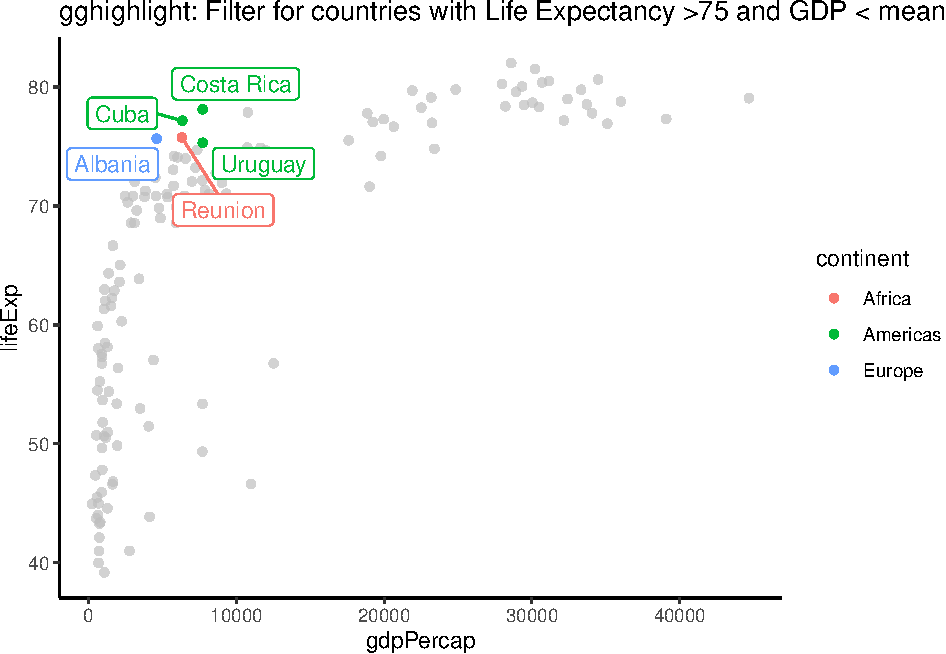
\includegraphics{cookbook_files/figure-latex/gghighlight-1.pdf}

\bibliography{book.bib,packages.bib}


\end{document}
